\chapter{Introducción específica} % Main chapter title

\label{Chapter2}

%----------------------------------------------------------------------------------------
%	SECTION 1
%----------------------------------------------------------------------------------------
En este capítulo se introduce la terminología específica de la red de comunicaciones del tren (TCN) y del sistema de información visual al pasajero (PIDS). La arquitectura del sistema y  sus módulos principales son presentados con una descripción general. Además, se introduce el sistema de carteles led de Trenes Argentinos, que son los que brindan información al pasajero en los coches de las formaciones ferroviarias operativas.\\


\section{Red de comunicación del tren TCN}

La red de comunicaciones del tren TCN presenta una arquitectura de buses jerárquicos de dos niveles, y está especificada en el estándar IEC-61375-1 \cite{IEC-61375-1999} de la \textit{International Electrotechnical Commission} (IEC). En la figura \ref{fig:redTCN} se presenta el esquema de conexión de los buses de datos de la TCN, el \textit{Wire Train Bus} (WTB) que se encarga de las comunicaciones entre coches a través de nodos con redundancia física, y el \textit{Multi Vehicle Bus} (MVB), al que se conectan los dispositivos de cada coche. 
Cada bus de datos tiene su especificación de detalle en las normas de la IEC \citep{CSN-EN-61375-2-1} y \citep{IEC-61375-3-1:2012}. \\

\begin{figure}[ht]
	\centering
	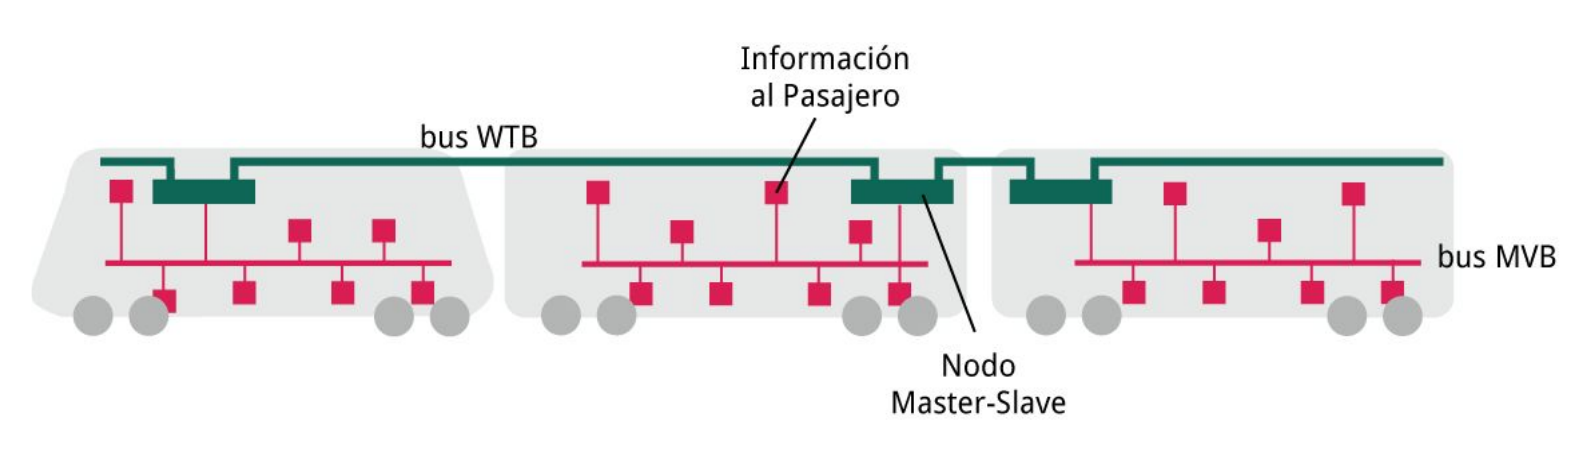
\includegraphics[width=1\textwidth]{./Figures/diagramaRedTCN.png}
	\caption{Diagrama del tren y de los buses WTB/MVB de la red TCN.}
	\label{fig:redTCN}
\end{figure}

En la figura \ref{fig:sofseTCN} se presenta la topología de la red TCN para los trenes de SOFSE. Se puede observar en el plano que los módulos se repiten en cada coche y, resaltado en celeste, la ubicación del sistema PIDS y CCTV en los coches cabecera. Algunos de los dispositivos y sistemas conectados al MVB son: el control de puertas (DOORL/R), el aire acondicionado (HVAC), el sistema de tracción (VVVF), el sistema de control de frenos (BCU), entre otros. El mapa de recorrido led, los carteles de matriz led, los parlantes (SPK) y las cámaras de video (CCTV), son parte del PIDS, que también se interconecta al bus MVB. 

\begin{figure}[hh]
	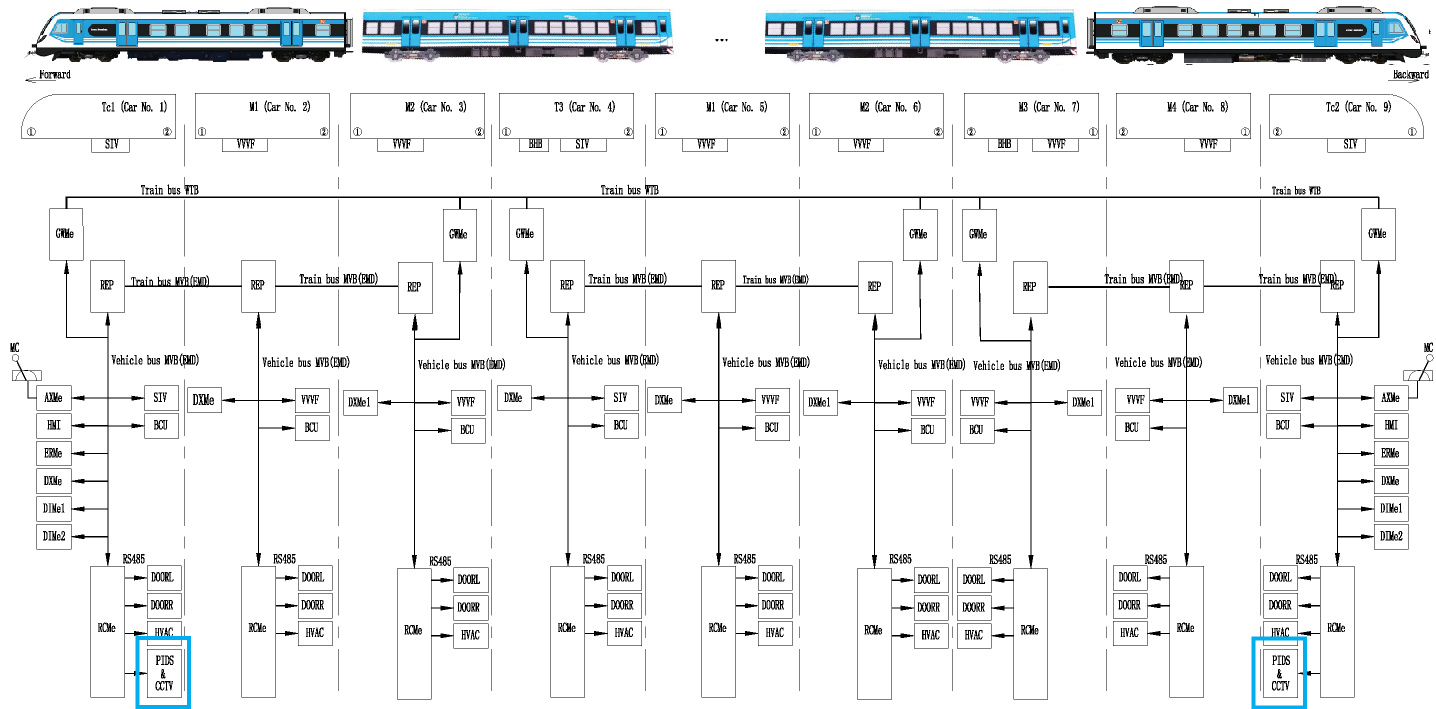
\includegraphics[width=1.75\textwidth, angle=90]{./Figures/diagramaTrenesArgentinosTCN2.png}
	\caption{diagrama de la red TCN de Trenes Argentinos. Plano cortesía SOFSE, editado por parte del autor.}
	\label{fig:sofseTCN}
\end{figure}

El PIDS se conecta a un módulo denominado RCMe, a través de una red RS485. Este último bloque se corresponde con un módulo específico de hardware instalado en los rack de salón, el RCMe, recuadrado en celeste en la figura \ref{fig:imgRackTCN}. En la figura, además de este módulo, se observan distintas unidades similares en las primeras filas del rack. En las últimas filas están los módulos correspondientes al PIDS, también resaltados en celeste.  \\

\begin{figure}[ht]
	\centering
	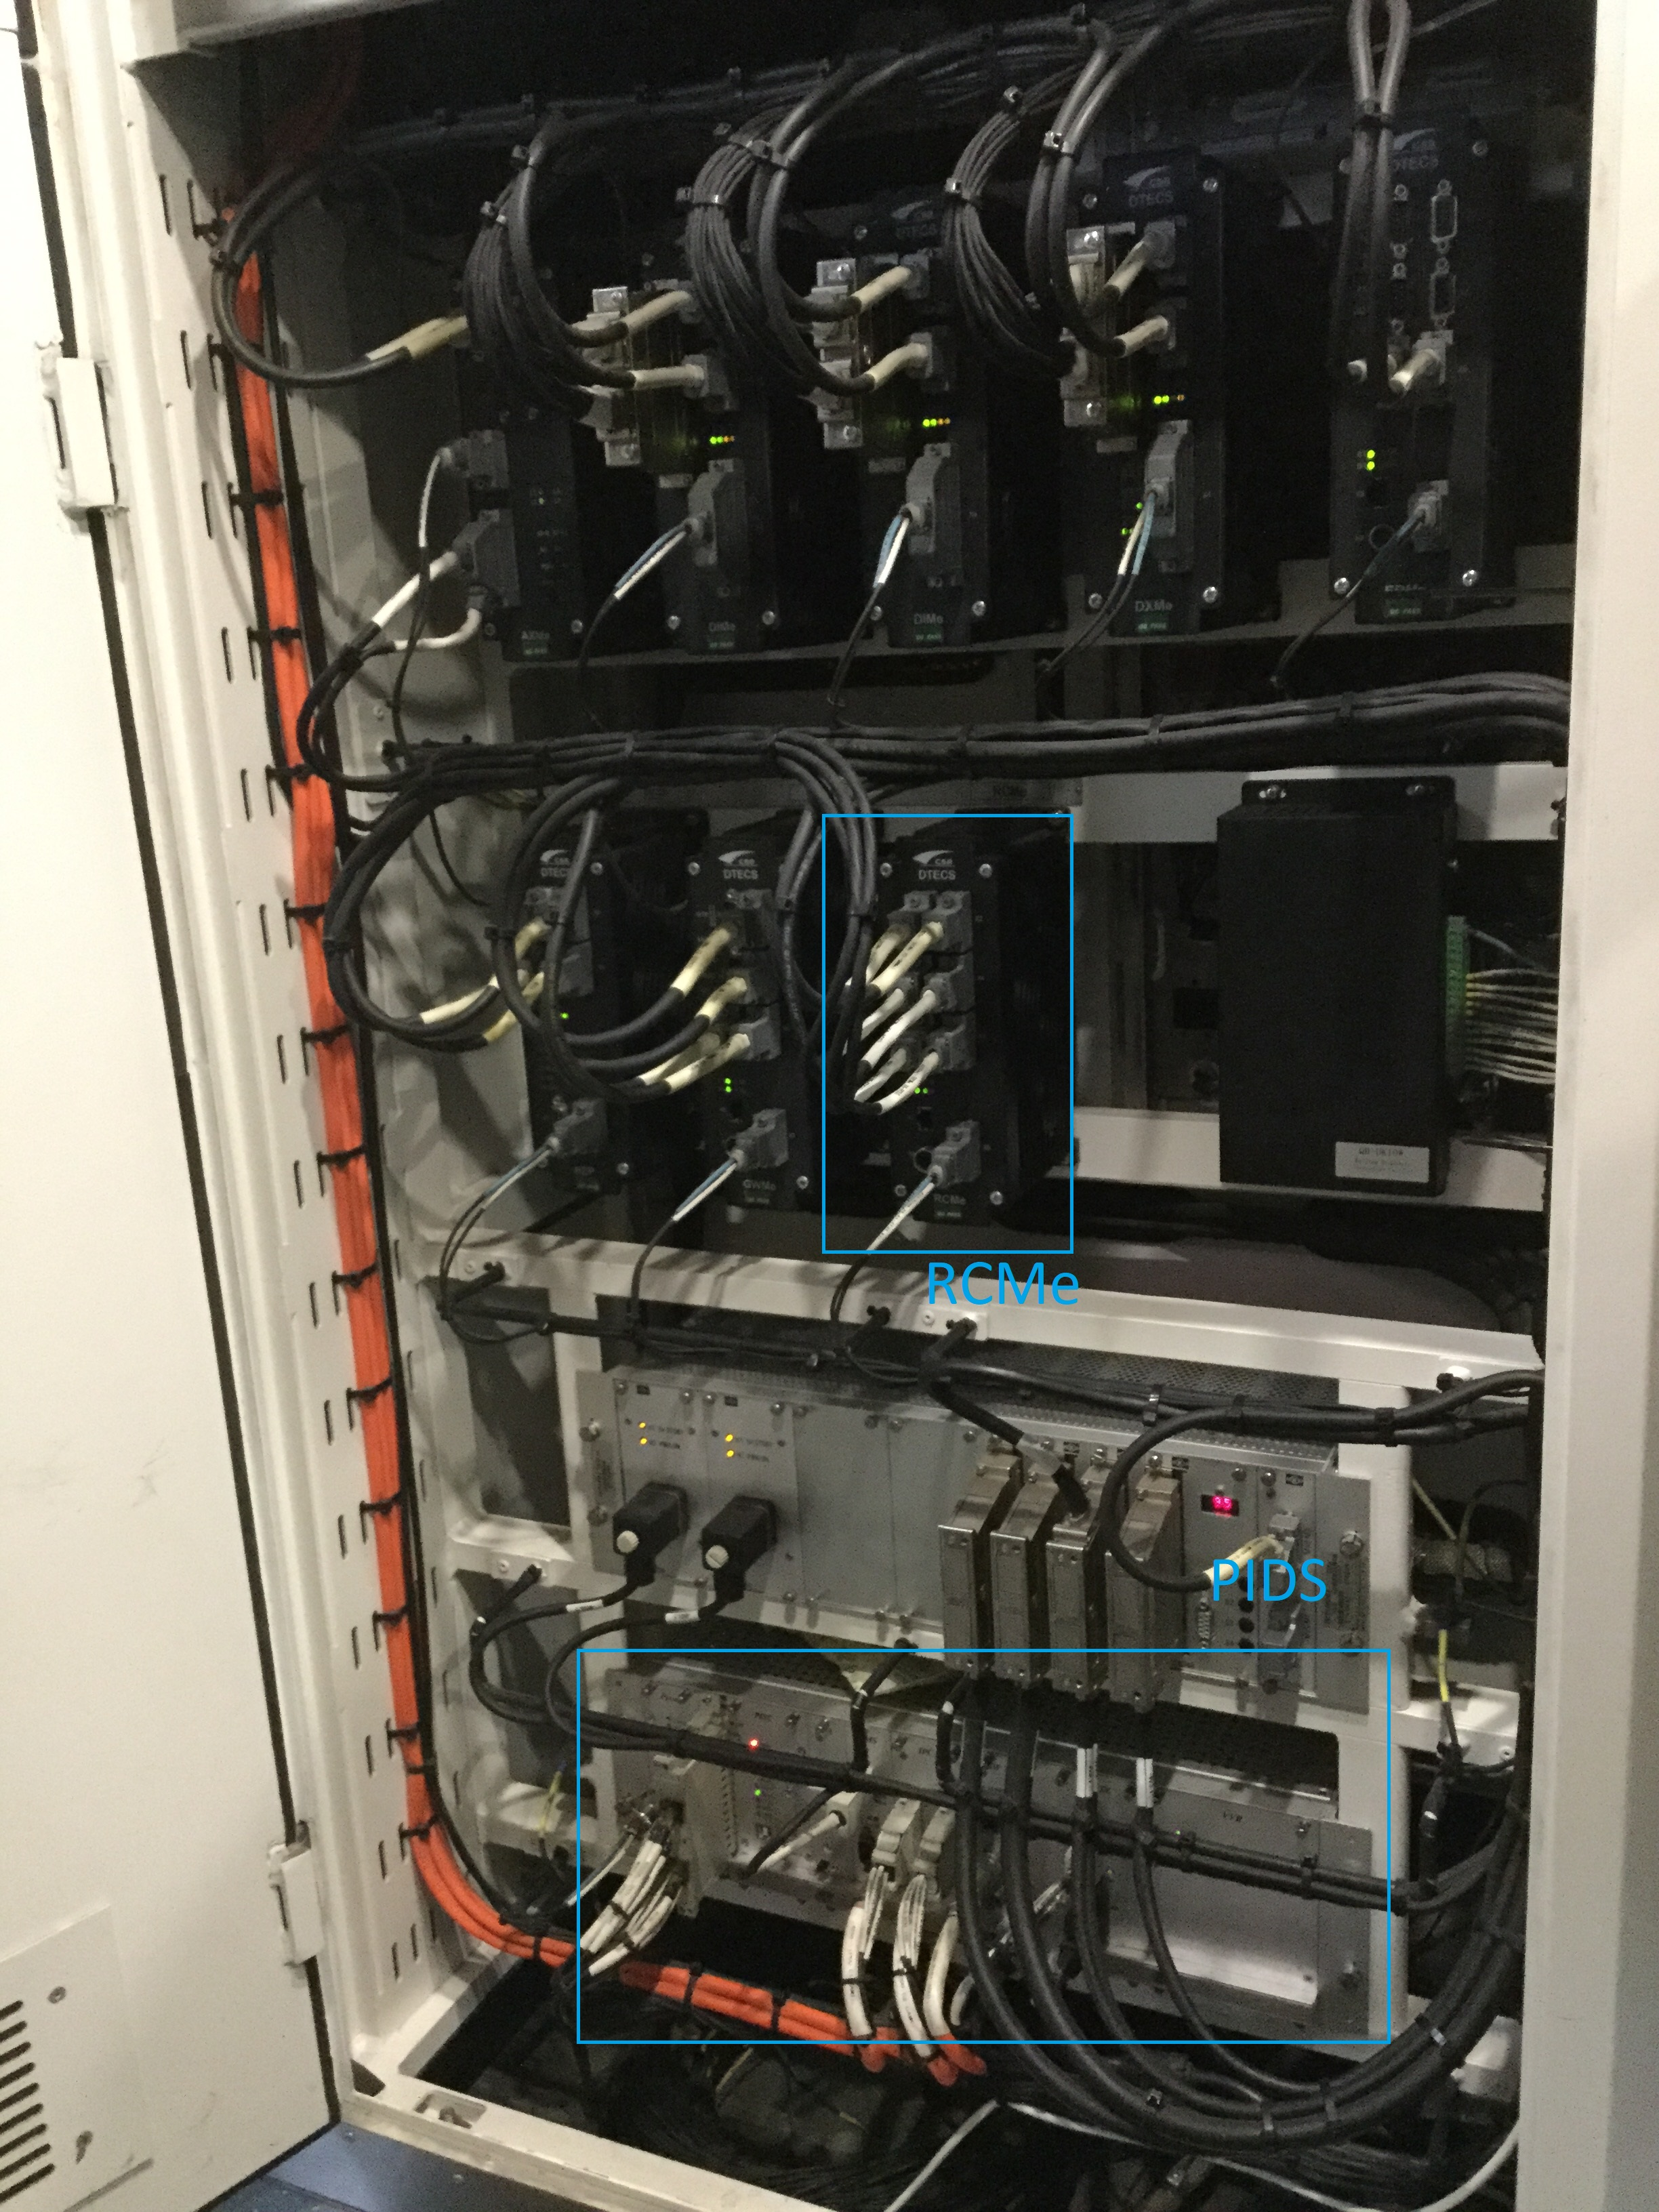
\includegraphics[width=0.75\textwidth , angle=0]{./Figures/imgRackTCN.JPG}
	\caption{Fotografía del rack de salón de una formación de Trenes Argentinos.}
	\label{fig:imgRackTCN}
\end{figure}

Los módulos negros que se observan en la figura \ref{fig:imgRackTCN} se denominan DIMe, DXMe y RCMe, y son parte de la solución TCN del Instituto Zhuzhou, denominada Distribute Train Electric Control System (DTECS)  \cite{feng2016survey}. Los módulos incluyen un gateway WTB/MVB. \\

\begin{figure}[h!]
	\centering
	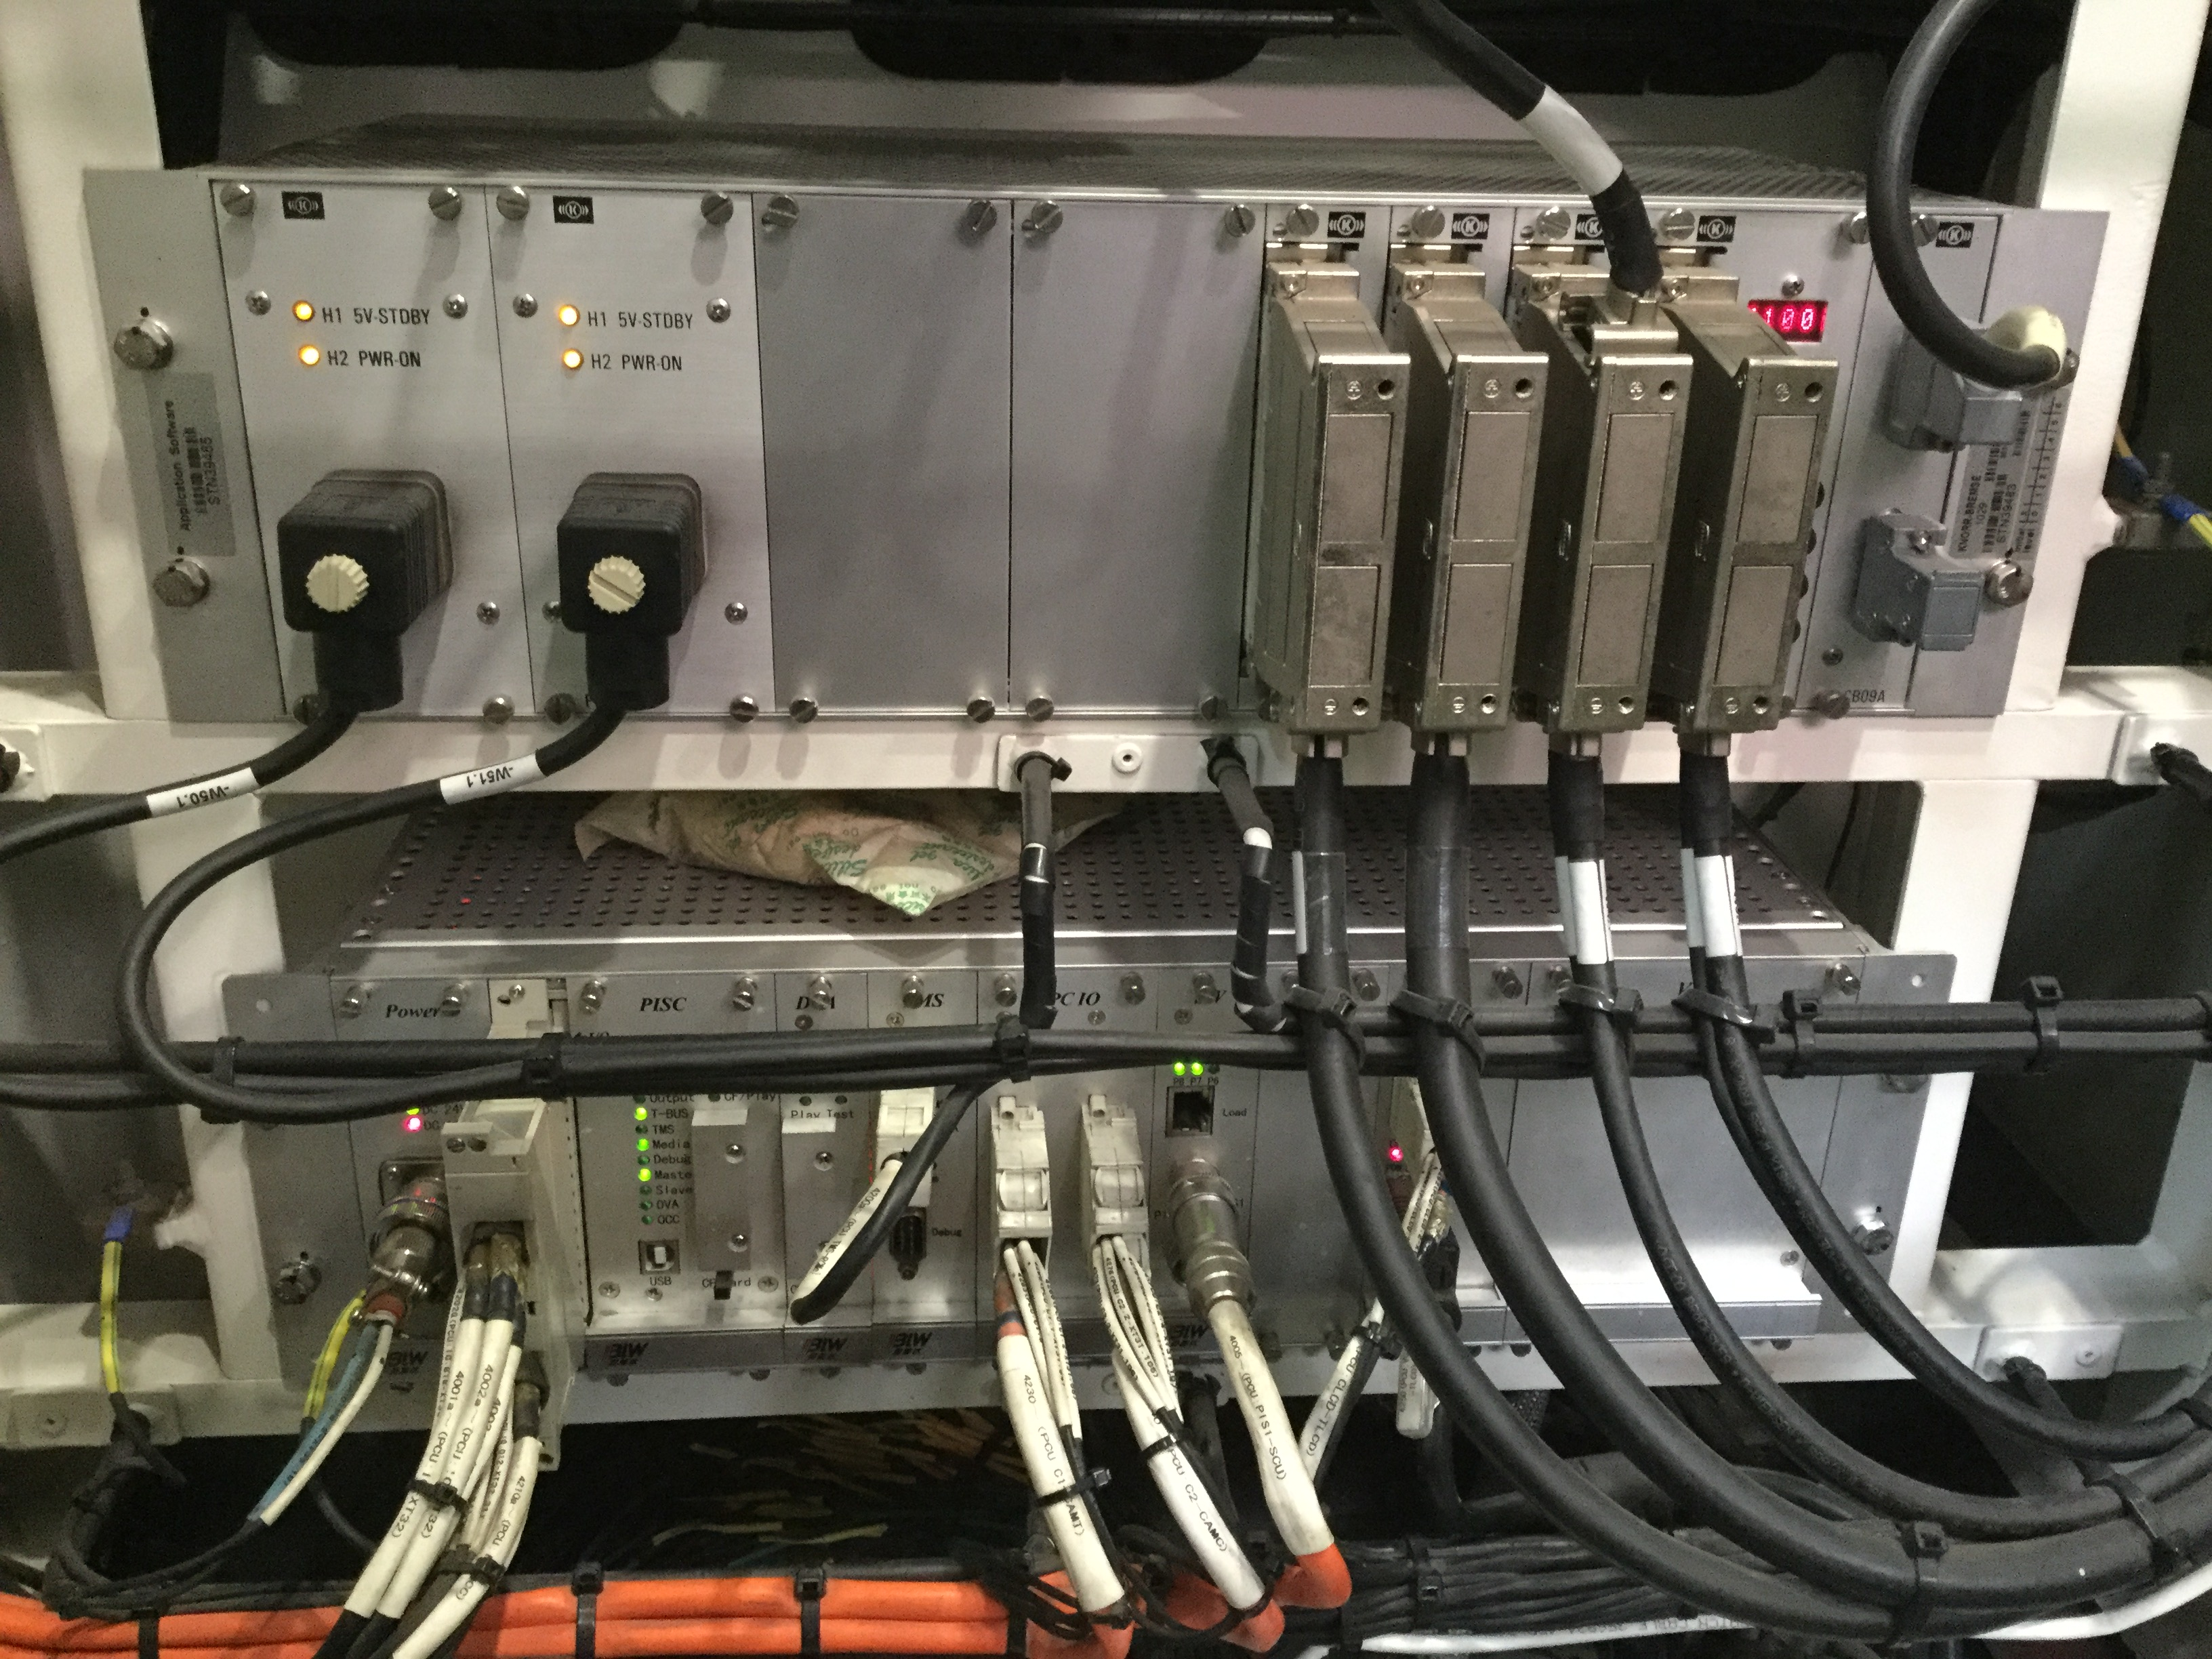
\includegraphics[width=0.75\textwidth]{./Figures/rackPIDS1.JPG}
	\caption{Fotografía de las unidades de rack del sistema PIDS en el rack de salón.}
	\label{fig:rackPIDS1}
\end{figure}

Según lo observado en las formaciones de Trenes Argentinos, y también en el plano de la red TCN, el PIDS tiene su propia red RS485. En la figura \ref{fig:rackPIDS1} se presenta un detalle de la unidad de rack donde están instalados sus módulos de hardware.\\

\pagebreak
\newpage

\section{PIDS: Sistema de información visual para pasajeros}

El PIDS de Trenes Argentinos es una solución propietaria, y no está especificada en ningún estándar. Este sistema integra un circuito cerrado de cámaras de TV (CCTV), un sistema de audio, mapas de recorrido y carteles led. En la figura \ref{fig:diagramaPIDS} se presenta su arquitectura.\\

\begin{figure}[ht]
	\centering
	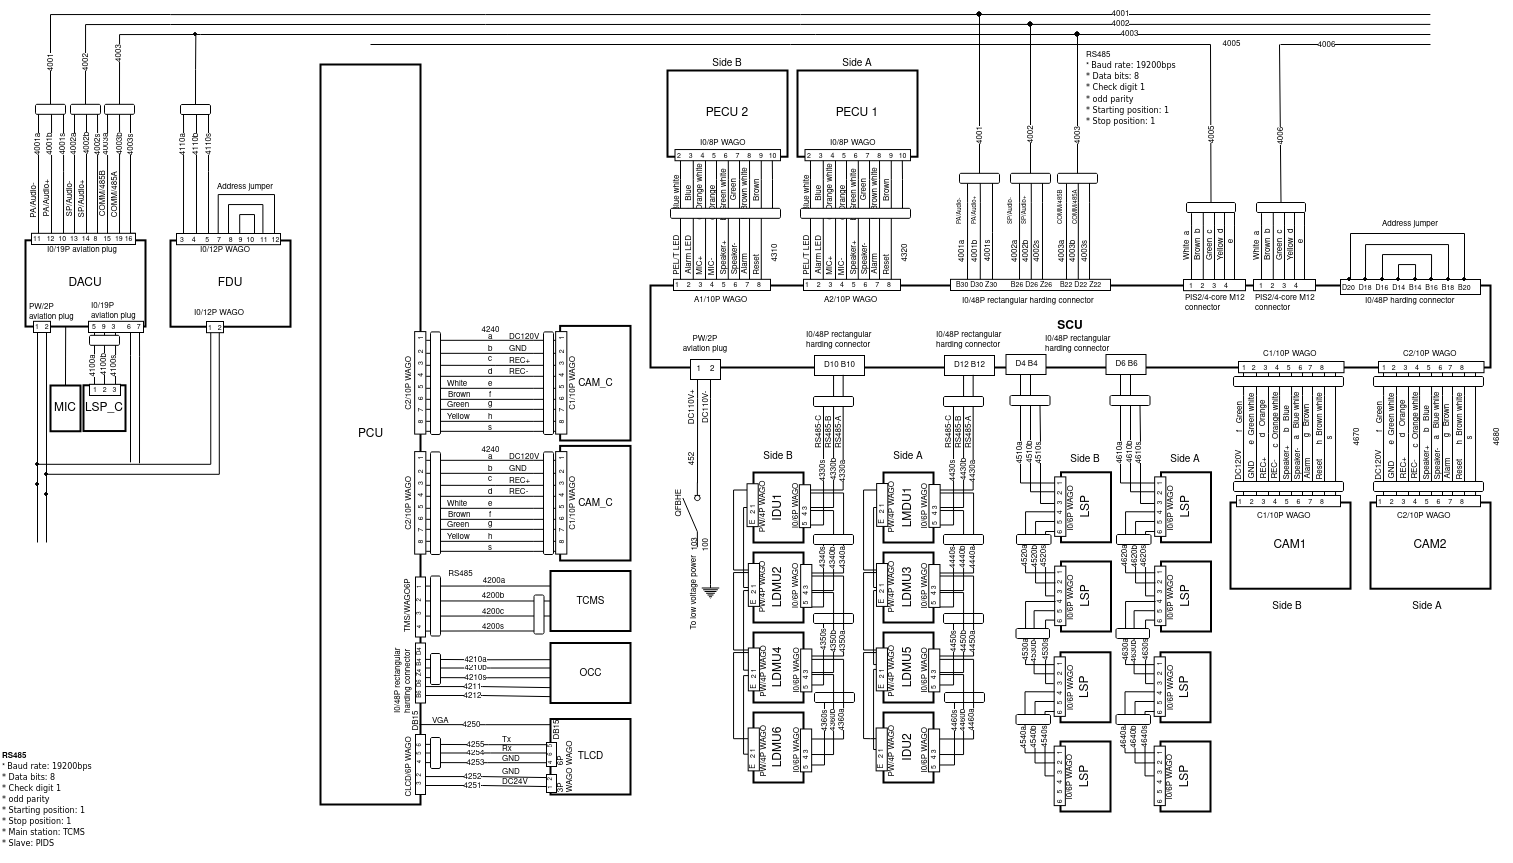
\includegraphics[width=1.66\textwidth, angle=90]{./Figures/diagramaPIDS.png}
	\caption{Diagrama de bloques del sistema PIDS, elaborado por el autor en base al plano de referencia de SOFSE.}
	\label{fig:diagramaPIDS}
\end{figure}

Este plano de referencia detalla importantes conexiones del sistema. Leyendo de izquierda a derecha en la dirección del plano, se pueden observar dos módulos denominados DACU y FDU, encargados del micrófono, del audio, de la comunicación con los sistemas CAM T, CAM C, TCMS, OCC y TLCD (pantalla LCD del conductor) a través del módulo vertical PCU, y de ser un extremo de conexión del bus de datos RS485 a través del cableado 4001, 4002 y 4003. Este bus de tres cables se interconecta a un módulo horizontal denominado SCU al que se conectan otra serie de módulos: PECU1 y PECU2 indicando referencia de los laterales del tren, CAM1 y CAM2, y cuatro arreglos serie de módulos. Dos de los módulos serie integran los bloques IDU (carteles de matriz led) y LDMU (mapas de recorrido led). Los otros dos módulos serie integran los bloques LSP o parlantes. Se puede observar que de estas conexiones serie hay dos módulos IDU: IDU1 al comenzar y IDU2 al finalizar el arreglo serie. Esto se corresponde con la distribución espacial de los carteles de matriz led en el salón de cada coche.\\



\section{Carteles y controladoras de matrices led}
En la sección del estado del arte de sistemas de información visual, se han presentado distintos tipos de carteles led y controladores asociados. Los carteles de matriz led de las formaciones de Trenes Argentinos están compuestos de módulos de 8x8 leds, que forman carteles de 48 módulos monocromo (rojo) para los carteles de salón y de 12 módulos bicolor (rojo-verde) de mayor tamaño para los carteles de frente y contrafrente del tren. Las placas de control de estos carteles tienen, por un lado, conexión eléctrica con la red de 110 VDC del tren, y por otro, un circuito de datos de 5 VDC que se comunica con el conjunto de chips digitales de los módulos 8x8. \\

Los módulos IDU corresponden a las unidades por las que se transmiten datos a los carteles de matriz led. En el SCU termina un conjunto de cables mediante un conector Harting IO/48 P, dentro El bus RS485 que conecta el SCU con las unidades IDU está compuesto por los cables nomenclados como 4330a (RS485A), 4330b (RS485B) y 4330c (RS485C). 

\begin{figure}[ht]
	\centering
	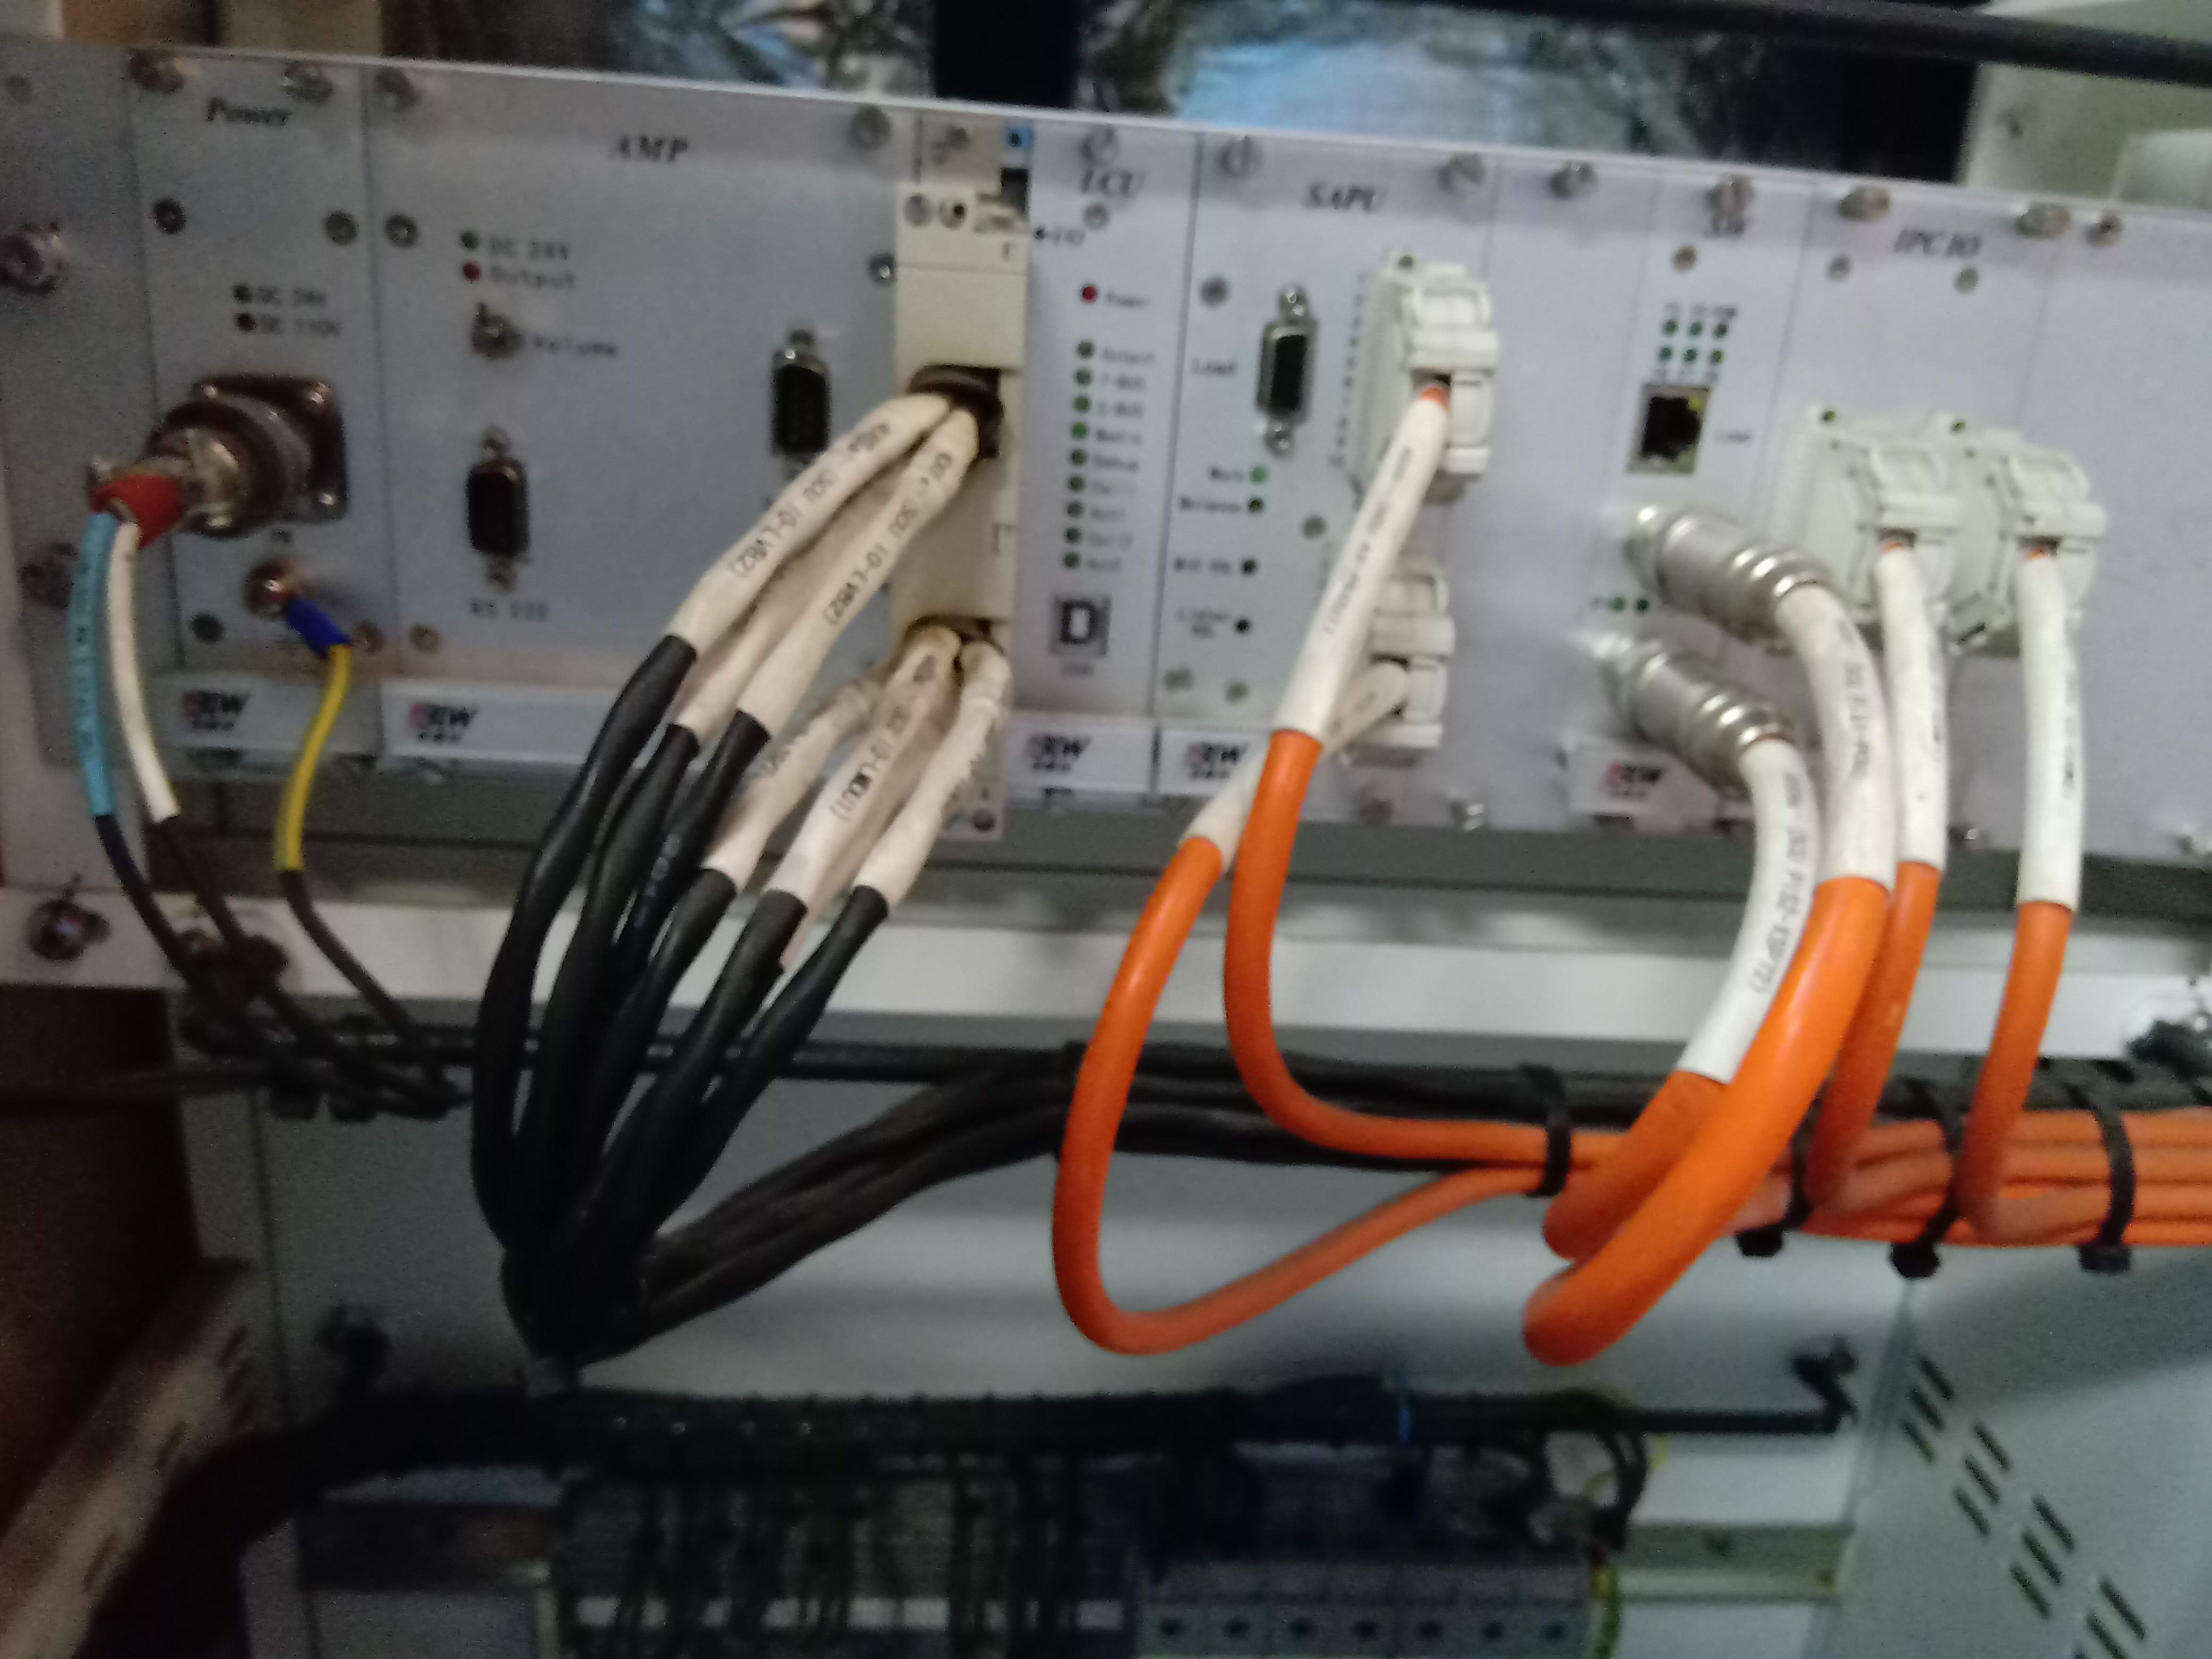
\includegraphics[width=1\textwidth ]{./Figures/rackPIDS2.jpg}
	\caption{Fotografía del detalle de cableado de la unidad de rack del PIDS que corresponde a los carteles LED de salón.}
	\label{fig:rackPIDS2}
\end{figure}



\begin{figure}[ht]
	\centering
	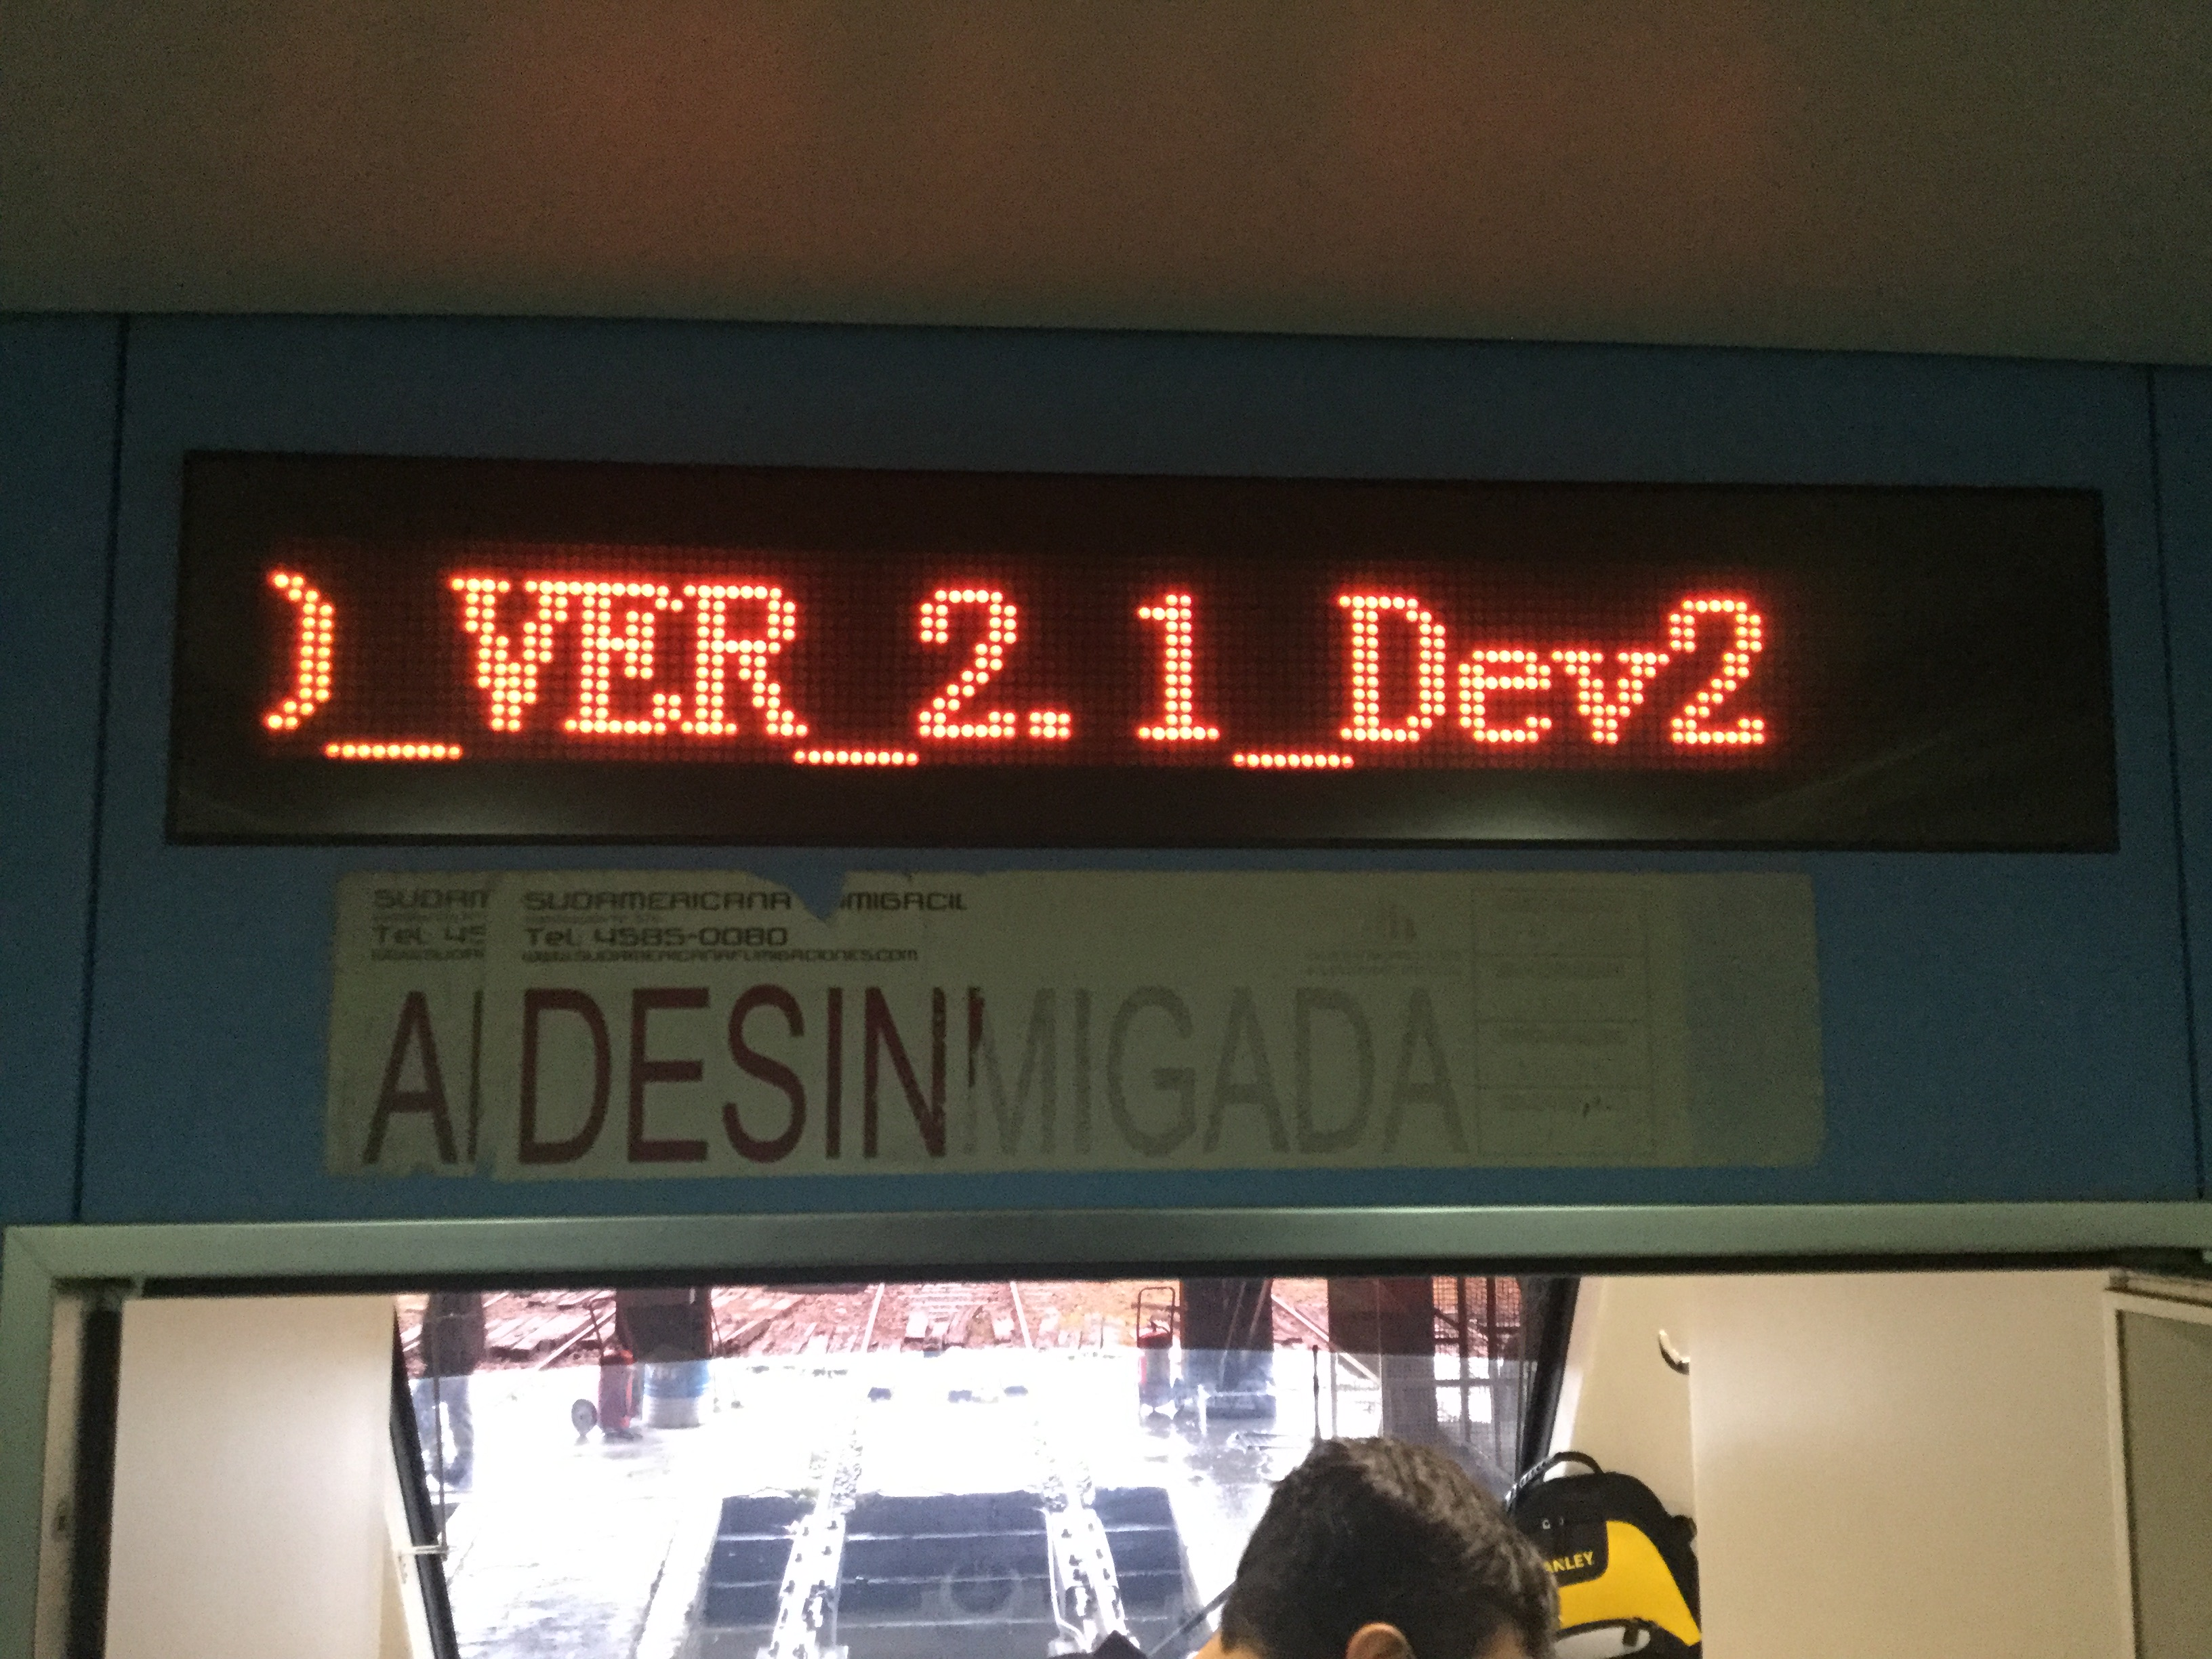
\includegraphics[width=1\textwidth]{./Figures/cartelIniciando.JPG}
	\caption{Fotografía de un cartel de salón inicializandose bajo una prueba de operación.}
	\label{fig:cartelIniciando}
\end{figure}

